        \chapter{Metode Penelitian}\label{ch:method}

    \section{Tahapan Penelitian}\label{sec:stages}
    Bab ini membahas metode yang digunakan dalam pelaksanaan penelitian Tugas Akhir. Penelitian ini mengimplementasikan algoritma genetika untuk optimasi parameter pada model yang memprediksi total \textit{revenue} (pendapatan) dari salah satu perusahaan SMS \textit{traffic management} di Indonesia. Tahapan penelitian pada Tugas Akhir ini ditunjukkan oleh Gambar 3.1 berikut.

    \begin{figure}[H]
        \centering
        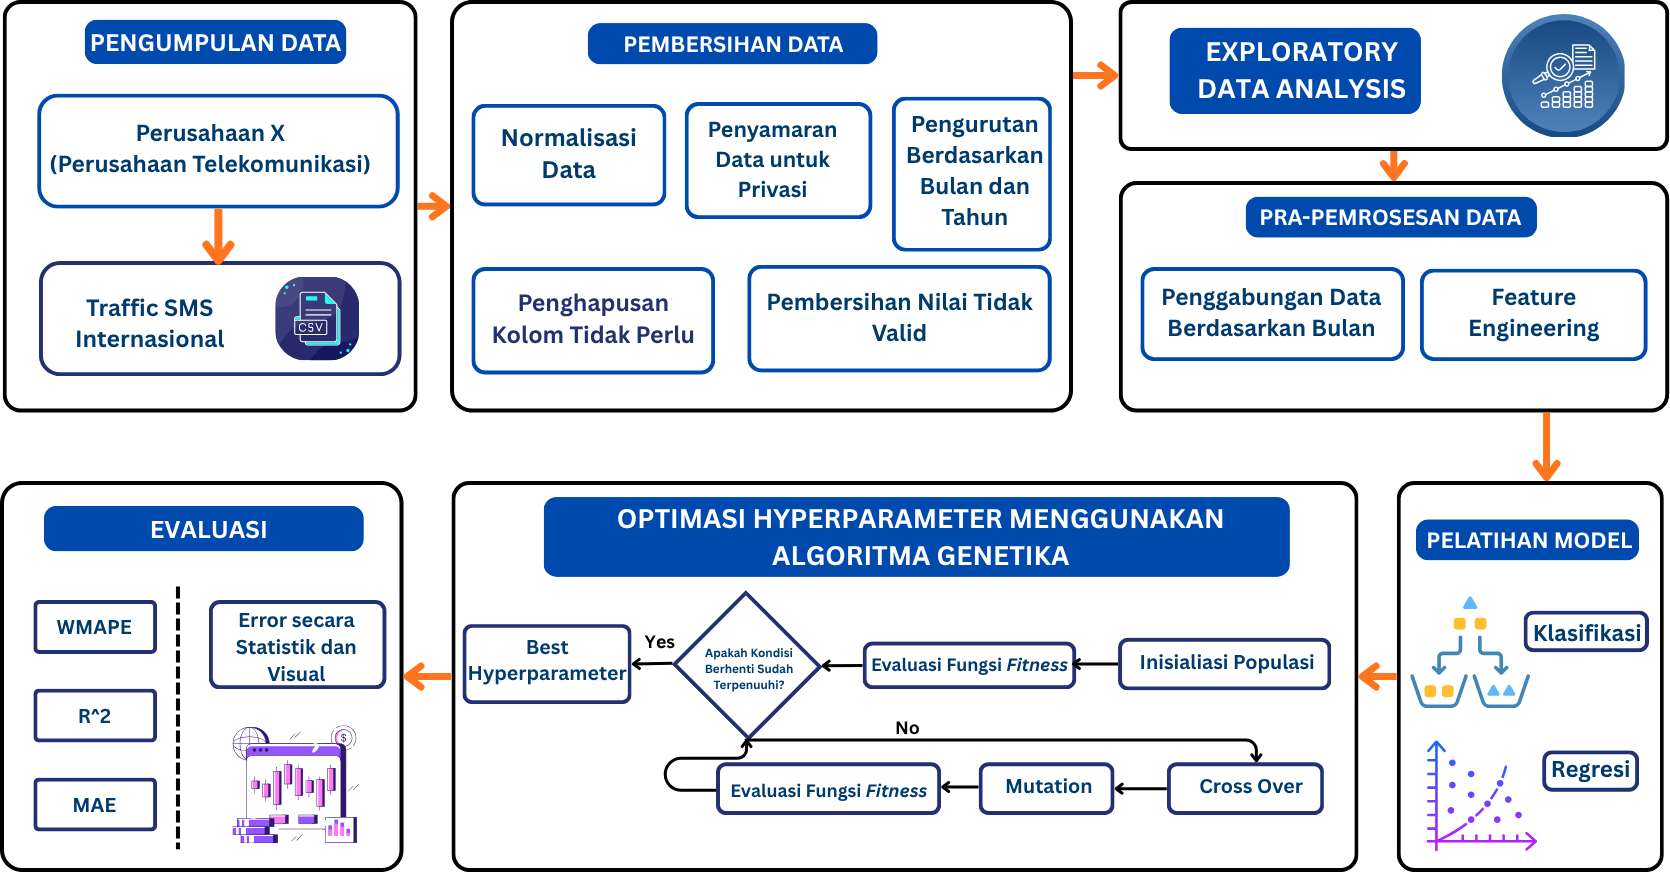
\includegraphics[width=0.9\textwidth]{tugas-akhir/assets/images/Diagram Alir Penelitian.png}
        \caption{Diagram Alir Penelitian}
        \label{fig:ga-flow}
    \end{figure}
    
    Tahapan penelitian dimulai dari pengumpulan data \textit{Traffic SMS Internasional} dari Perusahaan Telekomunikasi (X). Data tersebut kemudian dibersihkan (\textit{data cleaning}) dengan beberapa proses yaitu normalisasi data, penyamaran data untuk privasi, pengurutan data berdasarkan bulan dan tahun, pembersihan nilai tidak valid, serta penghapusan kolom data atau fitur yang tidak diperlukan. Kemudian dilakukan proses \textit{Exploratory Data Analysis} untuk mendapatkan \textit{insight} dari data. Selanjutnya dilakukan pra-pemrosesan data dengan menggabungkan data berdasarkan bulan data  dan pembuatan \textit{feature engineering}. Kemudian data dimasukkan dalam model prediksi untuk memprediksi kolom target yaitu \textit{TotalRevenue} dengan dua tahapan (\textit{two stage}) yaitu klasifikasi dan regresi. Klasifikasi bertujuan untuk memprediksi pendapatan yang nol dan tidak nol. Regresi bertujuan untuk memprediksi  pendapatan tidak nol di bulan selanjutnya dari hasil prediksi model klasifikasi. Model prediksi pada regresi dioptimasi dengan \textit{hypeparamater tuning} menggunakan Algoritma Genetika. Parameter terbaik akan digunakan dalam model untuk memprediksi \textit{TotalRevenue}. Hasil prediksi akan dievaluasi menggunakan metriks evaluasi yaitu WMAPE, MAE dan $R^2$ dan \textit{error} secara statistik dan visual.
    
    \section{Pengumpulan Data}\label{sec:data collection}
    Data yang digunakan dalam penelitian ini adalah data transaksi SMS A2P (\textit{Application to Person}) dari perusahaan X, salah satu perusahaan yang berfokus pada \textit{traffic management} pada lalu lintas SMS Internasional,  pada tahun 2023 sampai 2024. Data yang digunakan terdiri dari 94.335 data dengan 19 kolom, kolom fitur sebanyak 18 kolom  yaitu Year, Month, Client, ClientConnection, Supplier, SupplierConnection, SupplierConnectionLink, Route, Country, Network, OAProfiledCategory,  CostCurrency, PriceCurrency, ProfitCurrency, BaseCurrency, TotalCost, TotalSentMessages,TotalDeliveredMessages, TotalUndeliveredMessages dan kolom target yaitu TotalRevenue.

    \section{Pembersihan Data}\label{sec:preprocessing}
    Pembersihan data merupakan tahapan penting sebelum data digunakan dalam proses pelatihan model maupun optimasi hiperparameter. Tahapan ini bertujuan untuk memastikan bahwa data yang digunakan bersih, terstruktur, dan sesuai dengan kebutuhan algoritma. Pada penelitian ini, proses pembersihan data meliputi beberapa langkah, yaitu normalisasi data, pengurutan data berdasarkan waktu, penghapusan kolom yang tidak diperlukan, dan pembersihan nilai tidak valid. Berikut merupakan penjelasan rinci setiap tahapan.

    \subsection{Normalisasi Data}\label{}

    Dataset yang digunakan memiliki ketidaknormalan data dan duplikasi data akibat salah ketik. Oleh karena itu, untuk mengatasi hal ini, langkah awal pembersihan adalah menormalisasi data akibat salah ketik tersebut menjadi data yang benar sehingga data yang salah ketik tersebut tidak dianggap data yang berbeda oleh model. Tujuannya adalah untuk memastikan data yang diproses sudah benar dan memang tidak ada kesalahan ketik ketika nantinya dimasukkan ke model. Data yang salah ketik ini terdapat pada kolom kategorikal.

    \subsection{Penyamaran Data untuk Privasi}\label{}
    Data yang digunakan memiliki informasi nama perusahaan yang sensitif. Menurut perjanjian dengan perusahaan X, peneliti harus menyamarkan data yang terkait dengan nama perusahaan dan informasinya sehingga data tersebut disamarkan dengan menggunakan metode penyamaran deterministik. Metode yang digunakan untuk penyamaran adalah pemetaan deterministik (\textit{deterministic mapping}) sehingga data yang dipetakan akan konsisten di tiap kolom. Kolom-kolom yang diidentifikasi sensitif dan disamarkan yaitu \texttt{Client}, \texttt{ClientConnection}, \texttt{Supplier}, \texttt{SupplierConnection}, \texttt{SupplierConnectionLink}, \texttt{Route}, \texttt{Network}, dan \texttt{OAProfiledCategory}.
    
    \subsection{Pengurutan Data Berdasarkan Bulan dan Tahun}\label{}
    
    Data \textit{traffic} SMS internasional yang diperoleh dari Perusahaan X memiliki informasi waktu berupa bulan dan tahun. Oleh karena itu, langkah selanjutnya adalah mengurutkan data berdasarkan urutan kronologis. Tujuannya untuk memastikan analisis statistik dan eksplorasi data dilakukan secara berurutan, memudahkan pemetaan pola per bulan, dan mendukung proses pembagian data yang lebih representatif. Pengurutan dilakukan menggunakan kombinasi \textit{sort\_values} pada kolom waktu (misalnya \textit{Month} dan \textit{Year}).
    
    \subsection{Penghapusan Kolom yang Tidak Diperlukan}\label{} 
    
    Dataset awal memiliki sejumlah kolom yang tidak memiliki pengaruh signifikan terhadap model prediksi atau analisis. Pada tahap ini dilakukan penghapusan terhadap kolom kolom identitas yang tidak relevan, kolom yang tidak berhubungan dengan target (\textit{TotalRevenue}), serta kolom yang dapat menyebabkan data \textit{leak}. Penghapusan dilakukan untuk menyederhanakan dataset dan mengurangi kompleksitas model, sehingga proses \textit{training} menjadi lebih efisien.
    
    \subsection{Pembersihan Nilai Tidak Valid}\label{} 
    Tahap selanjutnya adalah pembersihan nilai yang tidak valid, seperti nilai nol yang tidak semestinya (misalnya \textit{TotalRevenue} tetapi bernilai 0), nilai negatif, entri kosong (\textit{missing values}), dan data inkonsisten akibat kesalahan input. Pembersihan data ini bertujuan untuk mengurangi \textit{noise} dan memastikan informasi yang ada di dataset relevan.
    
    \section{Exploratory Data Analysis \method}\label{sec:method construction}
    Selanjutnya dilakukan proses \textit{exploratory data analysis} untuk mengetahui pola dalam data seperti distribusi data, frekuensi tiap data dalam satu fitur, dan hubungan korelasi antara fitur numerik maupun kategorikal. Analisis dalam proses ini dilakukan dengan membuat berbagai macam \textit{chart} atau grafik visual dengan memanfaatkan library \textit{matplotlib} atau \textit{seaborn}. Analisis visual ini bermanfaat untuk membuat sebuah fitur baru seperti yang ada di proses sebelumnya dan proses pemilihan fitur (\textit{feature selection}). Proses \textit{feature selection} ini dapat dilakukan berdasarkan fitur-fitur yang memiliki korelasi tinggi dengan fitur target berdasarkan analisis visual yang dilakukan serta analisis berdasarkan pengetahuan domain tertentu (\textit{domain knowledge}). 

    
    \section{Pra-pemrosesan Data}\label{} 

    Setelah melakukan proses EDA untuk mengeksplorasi insight bisnis serta pola dari data dilakukan pra-pemrosesan data. Tahapan ini bertujuan  untuk memastikan data yang dimasukkan ke model dapat diprediksi dengan lebih mudah serta dengan pola yang didapatkan sebelumnya dapat ditentukan pra-pemrosesan data yang lebih sesuai. Pada penelitian Tugas Akhir ini, proses pra-pemrosesan data terdiri dari penggabungan data berdasarkan bulan, pembuatan dan \textit{feature engineering}. Berikut merupakan penjelasan rinci di setiap tahapan.

    
    \subsection{Penggabungan Data Berdasarkan Bulan}\label{}  

    Data digabung dengan menjumlahkan metriks utama yaitu \texttt{TotalRevenue}, \texttt{TotalCost}, \texttt{TotalProfit}, \texttt{TotalSentMessages}, \texttt{TotalDeliveredMessages}, dan \texttt{TotalUndeliveredMessages} dengan metode \textit{sum}. Kemudian penggabungan tersebut berdasarkan \texttt{Series\_ID}, \texttt{Year}, \texttt{Month} sehingga bisa dianggap sebagai penggabungan data perbulan. \texttt{Series\_ID} sendiri  merupakan kombinasi antara \texttt{Client}, \texttt{Route}, \texttt{SupplierConnection}, dan \texttt{Network}. Penggabungan juga mempertimbangkan fitur lain yaitu dengan penghitungan data unik dari kolom \texttt{OAProfiledCategory} dengan metode \textit{nunique} yang mana nantinya dihasilkan fitur baru yaitu \texttt{unique\_OA\_count}, banyaknya \textit{flag} data anomali dari fitur \texttt{is\_anomaly\_rev\_only} dan \texttt{is\_anomaly\_cost\_only} menghasilkan fitur \texttt{anomaly\_count} serta rasio data anomali dengan total baris per grup menghasilkan fitur \texttt{anomaly\_revenue\_pct}, pendapatan maksimum dan minimum per kategori OA (\texttt{OAProfiledCategory}) dalam setiap grup dihitung yang menghasilkan fitur \texttt{max\_OA\_revenue} dan \texttt{min\_OA\_revenue} yang mengukur heterogenitas sub-transaksi.

    \subsection{\textit{Feature Engineering}}\label{}  
    \textit{Feature engineering} adalah proses untuk mengekstraksi fitur baru ataupun memodifikasi fitur yang sudah ada agar model lebih mampu mempelajari pola dalam data. Beberapa langkah \textit{feature engineering} yang dilakukan antara lain pembentukan fitur \texttt{Series\_ID}, pembuatan fitur untuk berdasarkan pola yang ada di data dengan analisis \textit{domain knowledge}, pembuatan fitur rasio atau perbandingan \textit{cost} (\texttt{rate\_Cost}), penambahan fitur baru untuk menandai anomali atau \textit{outliers} pada data, pembuatan fitur berdasarkan pola dari data sebelumnya, pembuatan fitur temporal yang mempresentasikan dinamik perubahan bisnis secara bulanan. Proses \textit{feature engineering} ini ada yang dilakukan sebelum proses penggabungan data berdasarkan bulan ada juga yang setelah proses penggabungan data berdasarkan bulan. Namun kebanyakan proses yang dilakukan setelah proses penggabungan data berdasarkan bulan karena data setelah proses ini yang akan dimasukkan kedalam proses pelatihan model. Langkah ini meningkatkan representasi informasi pada dataset sehingga dapat memperbaiki performa model.

    \section{Pelatihan Model \method}\label{sec:method construction}
    Untuk menyelesaikan prediksi \textit{revenue} yang mana memiliki karakteristik data yang agak kompleks. Data dengan pengelompokan berdasarkan \textit{Series\_ID} belum tentu ada di tiap bulan sehingga perlu untuk memprediksi ada atau tidaknya transaksi di tiap bulan kedepan dari masing-masing \texttt{Series\_ID}. Setelah penggabungan data beradasarkan bulan, data dengan nilai transaksi yang ada di tiap bulan memiliki proporsi 47.49\% dari seluruh data atau 994 dari 2093 total data. Maka dari itu perlu proses klasifikasi untuk membedakan ada atau tidaknya transaksi di tiap bulan kedepan. Hasil prediksi dari proses klasifikasi dapat disimbolkan sebagai nilai $P$ dengan $P = 0$ menunjukkan tidak adanya transaksi dan $P=1$ menunjukkan adanya transaksi. Apabila data tersebut ada transaksi baru dijalankan proses regresi untuk memprediksi \texttt{TotalRevenue}. Maka dari itu, hasil akhir dapat dinyatakan sebagai hasil perkalian antara proses klasifikasi dan proses regresi sehingga apabila $P = 0$ maka hasil akhir juga bernilai 0 sedangkan jika $P = 1$ maka hasil akhir dapat dinyatakan sebagai hasil output dari proses regresi karena $P = 1$ $.$ output regresi $=$ output regresi. 
    Untuk pembagian data dari proses klasifikasi diambil 80 \% data untuk data train dan 20 \% data untuk data test dengan menggunakan metode \textit{time based split} yaitu pembagian data berdasarkan urutan dari waktu \textit{month} dan \textit{year}. Model yang digunakan adalah model XGBoost dan menggunakan parameter default yaitu \texttt{n\_estimators} = 1000, \texttt{learning\_rate} = 0.3, \texttt{num\_depth} = 6,  \texttt{subsamples} = 1, \texttt{colsample\_bytree} = 1, \textit{random\_state} = 42, \texttt{early\_stopping\_rounds} = 50, dan \texttt{verbose} = 0. Evaluasi model menggunakan ROC AUC karena data \textit{imbalance} untuk transaksi yang aktif dan tidak aktif. Kemudian untuk proses regresi menggunakan pembagian data yang sama dengan proses klasifikasi hanya saja model yang digunakan lebih beragam yaitu menggunakan model XGBoost dan Random Forest. Dengan parameter default masing-masing model untuk XGBoost menggunakan \texttt{random\_state} = 42 dan \textit{verbose} = 0 sedangkan Random Forest mengguakan \texttt{random\_state} = 42 dan \texttt{n\_jobs} = -1. Dalam proses ini proses optimasi hiperparameter \textit{tree-based models} juga dilakukan yang mana hasilnya nanti akan dibandingkan dengan \textit{baseline} yaitu pelatihan model dari masing-masing model yang ada di proses regresi dengan parameter default. Proses ini akan dijelaskan lebih lanjut di subbab berikutnya. 

    \section{Optimasi Hiperparameter Menggunakan Algoritma Genetika\method}\label{sec:method construction}\
    Untuk mendapatkan konfigurasi parameter terbaik, penelitian ini menggunakan Algoritma Genetika (\textit{Genetic Algorithm}), sebuah metode pencarian heuristik yang terinspirasi dari proses seleksi alam. Pendekatan ini dipilih karena kemampuannya yang superior dalam mengeksplorasi ruang pencarian parameter yang luas dibandingkan metode konvensional. Ruang pencarian parameter dapat dilihat pada Tabel 3.1. Ruang pencarian ini merujuk pada penelitian Mansoori (2023).
    
    \renewcommand{\arraystretch}{1.2}
    \begin{longtable}{l l l l >{\RaggedRight\arraybackslash}p{3cm}}
    \caption{Rentang Hiperparameter Model} \\
    \toprule
    \textbf{Model} & \textbf{Hiperparameter} & \textbf{Rentang} & \textbf{Tipe} & \textbf{Definisi} \\
    \midrule
    \endfirsthead
    \toprule
    \textbf{Model} & \textbf{Hiperparameter} & \textbf{Rentang} & \textbf{Tipe} & \textbf{Definisi} \\
    \midrule
    \endhead
    
    Random Forest & $n\_estimators$ & [50, 1000] & Integer & Jumlah pohon dalam ensemble \\
     & $max\_depth$ & [1, 7] & Integer & Kedalaman maksimum pohon \\
     & $min\_samples\_split$ & [2, 20] & Integer & Minimum sampel pemisahan node \\
     & $min\_samples\_leaf$ & [1, 50] & Integer & Minimum sampel pada daun \\
     & $max\_features$ & [1, 23] & Integer & Jumlah fitur yang dipertimbangkan \\
     & $max\_samples$ & [0.1, 1.0] & Float & Proporsi sampel untuk melatih tiap pohon \\
    \midrule
    XGBoost & $learning\_rate$ & [0.001, 1.0] & Float & Laju pembelajaran model \\
     & $n\_estimators$ & [50, 1000] & Integer & Jumlah iterasi boosting \\
     & $max\_depth$ & [1, 7] & Integer & Kedalaman maksimum pohon \\
     & $subsample$ & [0.1, 1.0] & Float & Proporsi sampel yang diambil \\
     & $colsample\_bytree$ & [0.1, 1.0] & Float & Proporsi fitur yang diambil \\
     & $reg\_lambda$ & [1, 3] & Float & Regularisasi L2 \\
    \bottomrule
    \end{longtable}
    \subsection{Representasi Kromosom}\label{sec:method construction}\
    Pada tahap ini, parameter \textit{tree-based models} direpresentasikan sebagai kromosom. Sesuai dengan penjelasan sebelumnya satu kromosom untuk Random Forest dan XGBoost sama - sama terdiri dari 6 gen. Karena kedua model dioptimalkan secara terpisah, setiap model memiliki representasi kromosom dan ruang pencarian masing-masing. Tiap gen tersebut masing-masing merepresentasikan satu hiperparameter. Setiap \textit{tree-based models} memiliki ruang pencarian yang akan dioptimalkan. Ruang pencarian ini dapat berupa rentang kontinu dan diskrit tergantung dari tipe data dari tiap parameter. Untuk lebih lengkapnya ruang pencarian Random Forest dapat dilihat pada Tabel \ref{tab:search_space_rf}.

    \begin{table}[H]
    \centering
    \caption{Ruang pencarian hiperparameter \textit{XGBoost}}
    \label{tab:search_space_rf}
    \begin{tabular}{llccc}
    \toprule
    \textbf{Gen} & \textbf{Hiperparameter} & \textbf{Tipe} & \textbf{Min} & \textbf{Maks} \\
    \midrule
    0 & \texttt{n\_estimators}       & Integer & 50    & 1.000 \\
    1 & \texttt{max\_depth}          & Integer & 1     & 7     \\
    2 & \texttt{min\_samples\_split} & Integer & 2     & 20    \\
    3 & \texttt{min\_samples\_leaf}  & Integer & 1     & 50    \\
    4 & \texttt{max\_features}       & Integer & 1     & 23 \\
    5 & \texttt{max\_samples}        & Float   & 0{,}1 & 1{,}0 \\
    \bottomrule
    \end{tabular}
    \end{table}
    
    Sama dengan kromosom \textit{Random Forest}, satu kromosom \textit{XGBoost} juga terdiri dari 6 gen. Tabel \ref{tab:search_space_rf} merangkum ruang pencarian \textit{XGBoost}. Proses dekode kromosom ke hiperparameter dilakukan melalui fungsi \texttt{decode\_rf()} dan \texttt{decode\_xgb()} yang masing-masing membulatkan nilai gen ke tipe data yang sesuai misalkan \textit{integer} atau \textit{float} dan memastikan berada dalam rentang yang valid melalui fungsi \texttt{np.clip()}.
    
    \subsection{Inisialisasi Populasi}\label{sec:method construction}\
    
    Pertama-pertama, populasi awal dinisiasi yang berisi sekumpulan kombinasi hiperparameter acak. Tujuan dari proses ini adalah untuk menciptakan solusi awal yang beragam sehingga dapat dieksplorasi oleh algoritma genetika. Ukuran populasi pada penelitian Tugas Akhir ini adalah 20. Dengan ukuran populasi tersebut terdiri dari 20 kromosom yang berbeda. Kemudian untuk \textit{random\_seed} diatur ke nilai 42 agar ditiap eksperimen yang dilakukan berulang dapat memiliki populasi awal yang sama. Tanpa pengaturan \textit{random\_seed} bisa berbeda di tiap eksperimen. Nilai 42 sendiri bukan ketentuan melainkan nilai yang popular digunnakan untuk \textit{data science} dalam mengatur nilai acak.

    \subsection{Evaluasi Fungsi \textit{Fitness}}\label{sec:method construction}\
    Pada setiap generasi, seluruh individu dalam populasi dievaluasi menggunakan fungsi objektif (\textit{objective function}) atau \textit{fitness function}. Pada penelitian ini, tujuan utama algoritma genetika adalah untuk meminimalkan kesalahan prediksi model. Oleh karena itu, \textit{objective function} dirancang menggunakan negasi dari metrik \textit{Weighted Mean Absolute Percentage Error} (WMAPE), yang mengukur kesalahan relatif antara nilai aktual dan nilai prediksi dengan mempertimbangkan bobot nilai aktual. Secara matematis, \textit{fitness function} dirumuskan pada persamaan 2.7. Proses negasi dilakukan karena GA pada library PyGad pada dasarnya berusaha memaksimalkan kromosom dengan nilai \textit{fitness} yang lebih tinggi sementara tujuan dari penelitian ini adalah untuk meminimalkan WMAPE. Pemilihan WMAPE didasarkan pada karakteristik data transaksi telekomunikasi yang memiliki \textit{sparsity} atau nilai nol pada variabel target, di mana apabila dibandingkan dengan penggunaan \textit{Mean Absolute Percentage Error} (MAPE) konvensional akan menghasilkan nilai tak terhingga (\textit{undefined}). WMAPE mengatasi masalah tersebut dengan menghitung total kesalahan absolut yang dibobotkan terhadap total nilai aktual, memberikan gambaran kesalahan secara agregat yang lebih representatif terhadap total omzet bisnis. 

    \subsection{Seleksi}\label{sec:method construction}\
    Pada proses seleksi, metode yang digunakan adalah metode \textit{tournament} yaitu individu dipilih secara acak dari populasi, lalu yang terbaik dari grup itu yang lolos menjadi parent. Metode ini dipilih karena metode ini cocok dengan range parameter yang lebar dan juga pendek di mana \textit{tree-based models} memiliki keragaaman \textit{range} parameter. Untuk parameter $k$ yang mempresentasikan jumlah anggota yang diambil acak di tiap grup diatur nilainya dengan $k = 3$. Nilai $k$ ini sudah sesuai karena tidak melebihi dari jumlah \textit{parents}(\textit{num\_parents\_mating}) yang akan diambil untuk dilakukan \textit{crossover}. Pada tahap ini jumlah \textit{parents} yang dipilih ditiap generasi yang dipresentasikan dalam PyGAD sebagai \textit{num\_parents\_matings} berjumlah 5.
    
    \subsection{\textit{Crossover}}\label{sec:method construction}\
    
    Selanjutnya reproduksi dilakukan tahap \textit{crossover} (kawin silang) untuk menggabungkan parameter secara acak dengan probabilitas kecil untuk menjaga keragaman populasi dan mencegah model terjebak pada solusi optimum lokal (\textit{local optima}). Dalam penelitian Tugas Akhir ini metode \textit{crossover} yang digunakan adalah \textit{uniform crossover}. Dengan pembentukan hasil dari kromosom anak (\textit{offsprings}) yang dapat dilihat pada persamaan 2.8 dan 2.9. Untuk probabilitas \textit{crossover} (\textit{crossover rate} pada penelitian ini ditentukan sebesar 1 di mana di tiap generasi pasti melakukan \textit{crossover}. 

    \subsection{\textit{Mutasi}}\label{sec:method construction}\

    Pada tahap mutasi, dilakukan proses perubahan pada gen di tiap kromosom untuk menjaga keragaman solusi. Probabilitas mutasi ($Pm$) yang digunakan sebesar 0.2 di mana 20\% dari jumlah gen akan dimutasi di tiap individu. Setelah jumlah gen yang dimutasi ditentukan, lokasi gen yang mengalami mutasi dipilih secara acak. Proses mtuasi dilakukan dengan menggunakan metode \textit{Random Mutation} dengan persamaan yang dapat dilihat pada persamaan 2.11. Setelah proses mutasi selesai, kromosom yang baru akan dievaluasi kembali fungsi \textit{fitness} nya dan dilakukan proses iterasi untuk pembentukan generasi baru begitu seterusnya sampai dengan jumlah generasi yang telah ditentukan. Kriteria penghentian ditentukan oleh jumlah generasi maksimum (50 generasi) dengan keep\_elitism = 2 yang memastikan 2 individu terbaik dari setiap generasi selalu dipertahankan tanpa modifikasi.
    
    \section{Evaluasi Hasil Optimasi Hiperparameter}

    Hasil optimasi hiperparameter kemudian dimasukkan ke dalam \textit{tree-based models} dan dievaluasi model tersebut untuk mengetahui performansinya terhadap data pendapatan layanan SMS internasional di perusahaan X. Dalam penelitian ini, sama dengan \textit{fitness function} metrik evaluasi utama yang digunakan adalah \textit{Weighted Mean Absolute Percentage Error} (WMAPE). 
    
    \begin{equation} \label{eq:r2}
    R^2 = 1 - \frac{\sum_{i=1}^{n} (y_{i} - \hat{y}_{i})^2}{\sum_{i=1}^{n} (y_{i} - \bar{y})^2}
    \end{equation}
    
    \begin{equation} \label{eq:mae}
    MAE = \frac{1}{n} \sum_{i=1}^{n} |y_{i} - \hat{y}_{i}|
    \end{equation}
    
    Selain WMAPE, penelitian ini juga menerapkan dua metrik pendukung lainnya, yaitu \textit{Coefficient of Determination} ($R^2$) dan \textit{Mean Absolute Error} (MAE). Koefisien determinasi ($R^2$) digunakan untuk mengukur proporsi varians dari variabel dependen yang dapat dijelaskan oleh model, di mana nilai yang mendekati 1 mengindikasikan kemampuan model yang sangat baik dalam menangkap pola data. Sementara itu, MAE digunakan untuk menghitung rata-rata selisih absolut antara nilai prediksi dan nilai aktual dalam satuan mata uang asli, yang memberikan interpretasi langsung mengenai besaran nominal kesalahan prediksi rata-rata per transaksi. Rumus untuk $R^2$ dan MAE ditunjukkan masing-masing pada Persamaan \ref{eq:r2} dan \ref{eq:mae}, di mana $y_i$ adalah nilai aktual, $\hat{y}_i$ adalah nilai prediksi, dan $\bar{y}$ adalah rata-rata nilai aktual.
    
    